\documentclass[11pt, a4paper]{article}
\usepackage{fontspec}
\usepackage{kotex}
\usepackage{amsmath, amssymb}
\usepackage{graphicx}
\usepackage{booktabs}
\usepackage{hyperref}
\usepackage{xcolor}
\usepackage{geometry}
\usepackage{listings}
\usepackage{float}
\usepackage{caption}
\usepackage{subcaption}

\geometry{margin=2.5cm}
\hypersetup{colorlinks=true, linkcolor=blue, urlcolor=blue}

\definecolor{pass}{RGB}{0,128,0}
\definecolor{warn}{RGB}{200,150,0}
\definecolor{fail}{RGB}{200,0,0}

\title{\textbf{SAM 3D Body 기반 7-View 투구 동작 재구성 리포트} \\
\large 다시점 마커리스 모션캡처 파이프라인 실행 결과}
\author{CJH}
\date{2026년 4월 14--15일}

\begin{document}
\maketitle
\tableofcontents
\newpage

% ============================================================
\section{개요}
% ============================================================

본 리포트는 SAM 3D Body (Meta, 2025)를 활용하여 7개 카메라(240Hz)의 야구 투구 영상에서 3D 인체 메시를 복원하고, 다시점 병합을 통해 정확한 SMPL 모션 파라미터를 추출하는 전체 파이프라인의 실행 결과를 기록한다.

\subsection{파이프라인 흐름}

\begin{center}
\begin{tabular}{c l l l}
\toprule
\textbf{Phase} & \textbf{단계} & \textbf{스크립트} & \textbf{상태} \\
\midrule
A & Bbox 추출 (로컬) & \texttt{00\_extract\_bbox\_crops.py} & \textcolor{pass}{완료} \\
A$'$ & SAM 3D Body 추론 (서버) & \texttt{01\_sam3d\_inference.py} & \textcolor{pass}{완료} \\
B & MHR$\to$Body25 변환 & \texttt{02a\_sam3d\_to\_keypoints.py} & \textcolor{pass}{완료} \\
C & 7-View 삼각측량 & \texttt{02b\_triangulate\_sam3d.py} & \textcolor{pass}{완료} \\
D & SMPL 초기화 피팅 & \texttt{02c\_init\_smpl\_from\_sam3d.py} & \textcolor{pass}{완료} \\
E & 7-View Reproj 최적화 & \texttt{02\_reproj\_7view\_sequential.py} & \textcolor{warn}{진행 중} \\
F & GART 포토메트릭 정제 & (다음 단계) & 대기 \\
\bottomrule
\end{tabular}
\end{center}

% ============================================================
\section{SAM 3D Body 소개}
% ============================================================

\subsection{모델 개요}

SAM 3D Body는 Meta Superintelligence Labs에서 개발한 단일 이미지 기반 3D 인체 복원 모델로, PA-MPJPE 30.4mm의 SOTA 성능을 달성한다. MHR (Momentum Human Rig) 127-관절 파라메트릭 바디 모델을 출력하며, 18,439개 정점의 고해상도 메시와 70개 키포인트를 생성한다.

\subsection{핵심 특징}
\begin{itemize}
    \item \textbf{단일 이미지 추론}: 카메라 캘리브레이션 없이 각 뷰에서 독립 추론
    \item \textbf{MHR 바디 모델}: 127 관절, 비선형 포즈 보정, LOD 시스템
    \item \textbf{DINOv3 백본}: Vision Transformer 기반 특징 추출
    \item \textbf{MoGe2 FOV 추정}: 프레임별 초점거리 자동 추정
    \item \textbf{내부 1.25$\times$ 패딩}: Tight bbox 입력 $\to$ 모델이 자동으로 25\% 확장
\end{itemize}

\subsection{MHR 70-Joint 구조}

\begin{center}
\begin{tabular}{c l | c l | c l}
\toprule
\textbf{Idx} & \textbf{관절} & \textbf{Idx} & \textbf{관절} & \textbf{Idx} & \textbf{관절} \\
\midrule
0 & Nose & 7 & L\_Elbow & 13 & L\_Ankle \\
5 & L\_Shoulder & 8 & R\_Elbow & 14 & R\_Ankle \\
6 & R\_Shoulder & 9 & L\_Hip & 41 & R\_Wrist \\
69 & Neck & 10 & R\_Hip & 62 & L\_Wrist \\
 & & 11 & L\_Knee & 15--20 & Feet (6) \\
 & & 12 & R\_Knee & 21--61 & Hands (40) \\
\bottomrule
\end{tabular}
\end{center}

\textbf{주의}: COCO/Body25와 인덱스 순서가 다름. 특히 Wrist가 41(R), 62(L)에 위치.

% ============================================================
\section{Phase A: Bbox 추출 \& SAM 3D Body 추론}
% ============================================================

\subsection{Tight Bbox 전략}

SAM 3D Body는 내부적으로 bbox에 1.25$\times$ 패딩을 적용한다. 따라서 입력 bbox는 \textbf{패딩 없이 마스크 contour에 밀착}해야 한다. 이를 위해 기존 SAM3 세그멘테이션 마스크에서 tight bbox를 추출했다.

\begin{center}
\begin{tabular}{l r r r}
\toprule
& \textbf{기존 (1.25$\times$ 패딩)} & \textbf{Tight (패딩 없음)} & \textbf{비율} \\
\midrule
cam3 평균 면적 & 134,547 px$^2$ & 86,106 px$^2$ & 1.56$\times$ \\
cam1 평균 면적 & 328,300 px$^2$ & 210,156 px$^2$ & 1.56$\times$ \\
\bottomrule
\end{tabular}
\end{center}

기존 패딩 bbox를 사용했다면 모델 내부 1.25$\times$와 합쳐져 \textbf{총 1.56$\times$ 이중 패딩}이 발생하여 인체 비율이 축소되었을 것이다.

\begin{figure}[H]
    \centering
    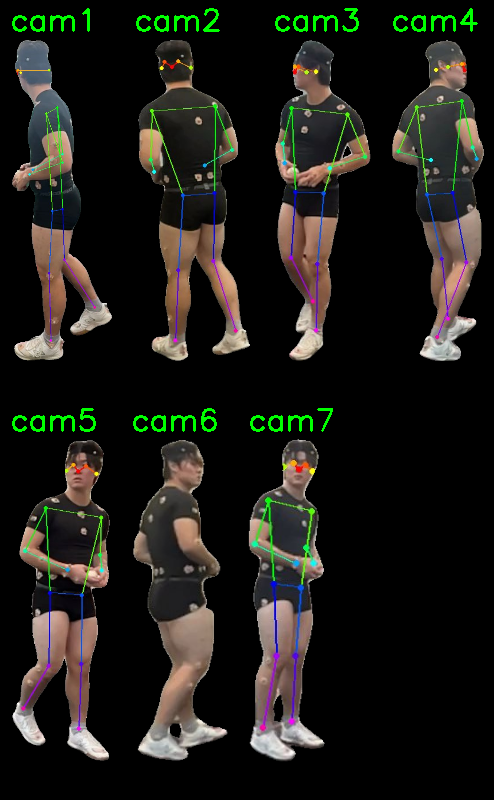
\includegraphics[width=0.7\textwidth]{figures/sam3d/all_cams_masked_bbox.png}
    \caption{7카메라 마스킹 + tight bbox 크롭 결과 (frame 0). 배경 완전 제거, 투구자만 추출.}
    \label{fig:masked_bbox}
\end{figure}

\subsection{SAM 3D Body 서버 실행}

\begin{center}
\begin{tabular}{l r r r r}
\toprule
\textbf{항목} & \textbf{값} & & \textbf{항목} & \textbf{값} \\
\midrule
서버 GPU & A100 80GB & & Conda env & sam3d (Python 3.11) \\
모델 & sam-3d-body-dinov3 & & 체크포인트 & 2.7 GB (HF gated) \\
Detector & 비활성화 (bbox 직접 제공) & & FOV & MoGe2 (자동) \\
\bottomrule
\end{tabular}
\end{center}

\subsection{추론 결과}

\begin{center}
\begin{tabular}{l r r r r}
\toprule
\textbf{카메라} & \textbf{프레임} & \textbf{시간} & \textbf{FPS} & \textbf{에러} \\
\midrule
cam1 & 999 & $\sim$12분 & 1.18 & 0 \\
cam2 & 999 & $\sim$12분 & 1.20 & 0 \\
cam3 & 1000 & 12분 14초 & 1.36 & 0 \\
cam4 & 1000 & 12분 38초 & 1.32 & 0 \\
cam5 & 1000 & $\sim$12분 & 1.33 & 0 \\
cam6 & 1000 & 11분 49초 & 1.41 & 0 \\
cam7 & 1000 & 11분 52초 & 1.40 & 0 \\
\midrule
\textbf{Total} & \textbf{6,998} & \textbf{83.4분} & \textbf{1.36 avg} & \textbf{0} \\
\bottomrule
\end{tabular}
\end{center}

\subsection{출력 데이터 구조}

각 프레임 \texttt{.npz} 파일에 저장된 키:

\begin{center}
\begin{tabular}{l l l}
\toprule
\textbf{Key} & \textbf{Shape} & \textbf{설명} \\
\midrule
\texttt{pred\_vertices} & (18439, 3) & MHR 메시 정점 \\
\texttt{pred\_keypoints\_2d} & (70, 2) & 이미지 평면 2D 키포인트 \\
\texttt{pred\_keypoints\_3d} & (70, 3) & 카메라 공간 3D 키포인트 \\
\texttt{body\_pose\_params} & (133,) & MHR 포즈 파라미터 \\
\texttt{shape\_params} & (45,) & MHR 체형 파라미터 \\
\texttt{focal\_length} & scalar & MoGe2 추정 초점거리 \\
\texttt{pred\_cam\_t} & (3,) & 약원근 카메라 translation \\
\texttt{bbox} & (4,) & 사용된 bbox [x1,y1,x2,y2] \\
\bottomrule
\end{tabular}
\end{center}

\subsection{MHR 메시 오버레이 시각화}

\begin{figure}[H]
    \centering
    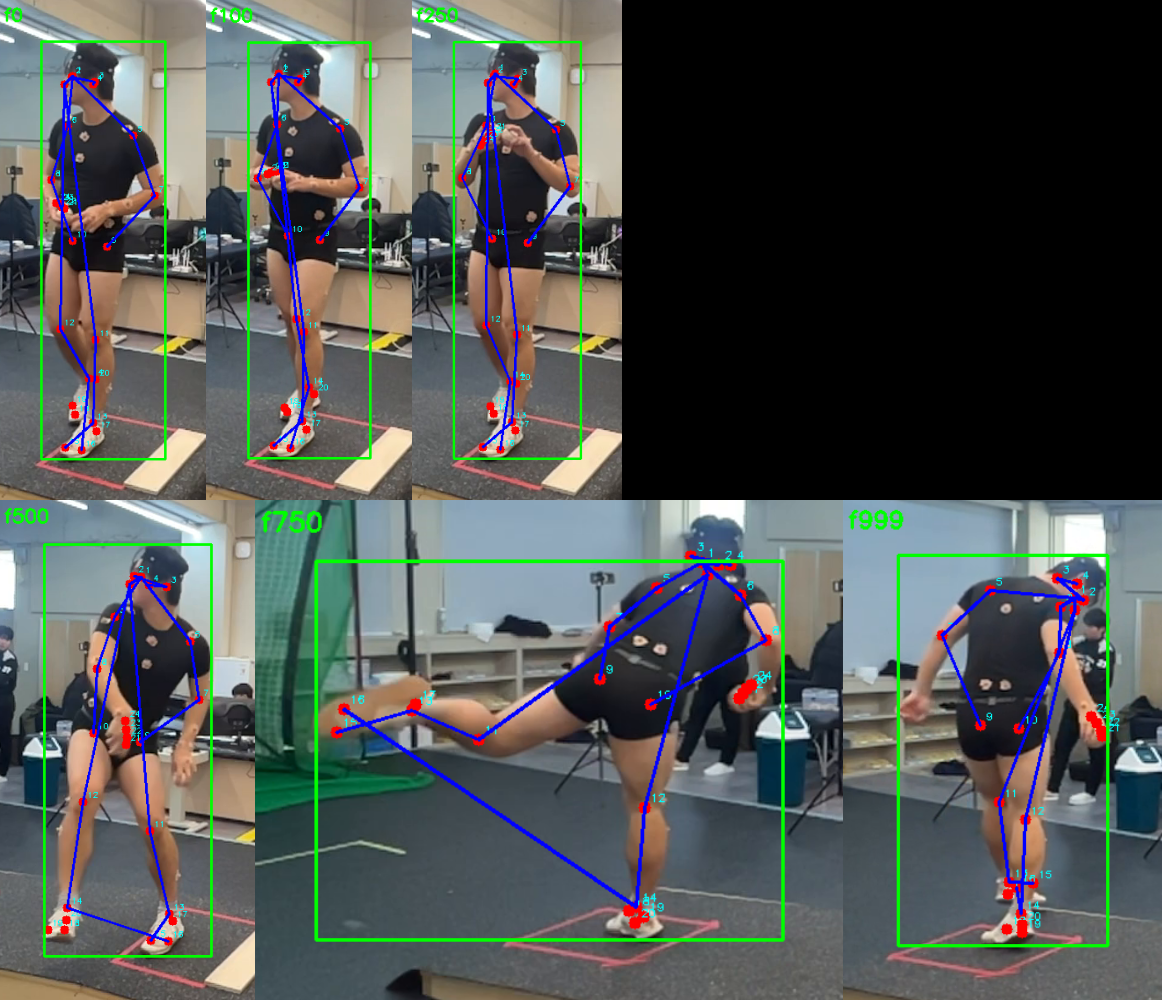
\includegraphics[width=0.85\textwidth]{figures/sam3d/cam3_keypoints_sample.png}
    \caption{cam3 SAM 3D Body 결과: MHR 70-joint 키포인트 + bbox 오버레이. 6프레임 샘플 (f0, f100, f250, f500, f750, f999). 투구 와인드업$\to$릴리스 전체 동작 포착.}
    \label{fig:cam3_keypoints}
\end{figure}

\subsection{후처리: 스무딩 \& Focal 고정}

SAM 3D Body는 프레임별 독립 추론이므로 두 가지 후처리를 적용했다:

\begin{enumerate}
    \item \textbf{Focal length 고정}: MoGe2가 프레임마다 다른 focal을 추정하여 메시 크기가 ``울렁거림''. 고정 렌즈이므로 전체 프레임 median focal로 고정.
    \item \textbf{Savitzky-Golay 스무딩}: 18,439 정점 $\times$ 3축 + camera translation에 Savgol filter (window=15, poly=3) 적용.
\end{enumerate}

\begin{center}
\begin{tabular}{l r r r}
\toprule
\textbf{카메라} & \textbf{Focal (원래)} & \textbf{Focal (고정)} & \textbf{Jitter 감소} \\
\midrule
cam1 & 729--776 & 753 & 59\% \\
cam2 & 759--782 & 769 & 52\% \\
cam3 & 760--795 & 781 & 52\% \\
cam4 & 765--812 & 783 & 51\% \\
cam5 & 744--767 & 755 & 57\% \\
cam6 & 764--787 & 776 & 63\% \\
cam7 & 740--761 & 749 & 64\% \\
\midrule
\textbf{평균} & & & \textbf{57\%} \\
\bottomrule
\end{tabular}
\end{center}

% ============================================================
\section{Phase B: MHR 70-Joint $\to$ OpenPose Body25 변환}
% ============================================================

SAM 3D Body의 MHR 70-joint 키포인트를 기존 파이프라인(\texttt{02\_reproj})이 소비하는 OpenPose Body25 형식으로 변환했다.

\subsection{매핑 테이블}

\begin{center}
\begin{tabular}{c l c l}
\toprule
\textbf{Body25} & \textbf{이름} & \textbf{MHR idx} & \textbf{비고} \\
\midrule
0 & Nose & 0 & \\
1 & Neck & 69 & \\
2 & R\_Shoulder & 6 & \\
3 & R\_Elbow & 8 & \\
4 & R\_Wrist & 41 & \textbf{$\neq$ COCO(4)} \\
5 & L\_Shoulder & 5 & \\
6 & L\_Elbow & 7 & \\
7 & L\_Wrist & 62 & \textbf{$\neq$ COCO(7)} \\
8 & MidHip & avg(9,10) & 합성 \\
9--14 & R/L Hip, Knee, Ankle & 10,12,14,9,11,13 & \\
\bottomrule
\end{tabular}
\end{center}

\textbf{결과}: 7카메라 $\times$ 999--1000프레임, 에러 0건. 출력: \texttt{sam3d\_kp\_body25/cam\{1-7\}/frame\_*.json}

% ============================================================
\section{Phase C: 7-View DLT 삼각측량}
% ============================================================

\subsection{방법}

7개 카메라의 Body25 2D 키포인트를 VGGT 캘리브레이션(K, R, t)을 사용하여 DLT (Direct Linear Transform) 삼각측량으로 월드 프레임 3D 관절 좌표를 계산했다.

\begin{itemize}
    \item 최소 3개 뷰에서 관측된 관절만 삼각측량 (\texttt{min\_views=3})
    \item 2$\sigma$ 이상치 제거 후 재삼각측량
    \item cam6 왜곡 보정: COLMAP k1=$-$0.346 적용
\end{itemize}

\subsection{캘리브레이션 선택: VGGT}

\begin{center}
\begin{tabular}{l l l}
\toprule
& \textbf{VGGT} & \textbf{COLMAP Rd2} \\
\midrule
Focal length & $\sim$734px (일관적) & 531--1367px (2.6$\times$ spread) \\
검증 여부 & 4-view reproj 성공 & 미검증 \\
신뢰도 & \textcolor{pass}{높음} & \textcolor{fail}{낮음} \\
\bottomrule
\end{tabular}
\end{center}

\subsection{결과}

\begin{center}
\fcolorbox{pass}{white}{\parbox{0.6\textwidth}{
\centering
\textbf{G1 게이트: \textcolor{pass}{PASS}} \\[4pt]
바디 관절 (0--14) 평균 리프로젝션 에러: \textbf{16.3px} (기준: $<$30px) \\
커버리지: \textbf{100.0\%} (모든 프레임, 모든 관절)
}}
\end{center}

\begin{center}
\begin{tabular}{l r}
\toprule
\textbf{지표} & \textbf{값} \\
\midrule
총 프레임 & 999 \\
관절당 유효 뷰 수 & 7/7 (전부) \\
평균 reproj error (body) & 16.3px \\
최대 reproj error (body) & $\sim$23px \\
이상치 비율 & 0\% \\
\bottomrule
\end{tabular}
\end{center}

\subsection{3D 뷰어}

삼각측량 결과 + MHR 포인트 클라우드를 Three.js 기반 인터랙티브 HTML 뷰어로 시각화했다 (\texttt{mhr\_3d\_viewer.html}). 마우스 드래그로 회전, 스크롤로 줌, Raw/Smoothed 실시간 전환 기능 포함.

% ============================================================
\section{Phase D: SMPL 초기화 피팅}
% ============================================================

\subsection{방법}

삼각측량된 3D 관절 좌표 (15개 Body25 관절)에 SMPL 모델을 3단계로 피팅:

\begin{center}
\begin{tabular}{c l l r r}
\toprule
\textbf{Stage} & \textbf{파라미터} & \textbf{설명} & \textbf{Steps} & \textbf{LR} \\
\midrule
1 & global\_orient + transl & 전역 회전 + 위치 & 100 & 0.02 \\
2 & + body\_pose (69) & 23개 관절 회전 & 300 & 0.01 \\
3 & + betas (10) & 체형 (매 10프레임) & 150 & 0.005 \\
\bottomrule
\end{tabular}
\end{center}

\subsection{결과}

\begin{center}
\begin{tabular}{l r}
\toprule
\textbf{지표} & \textbf{값} \\
\midrule
총 프레임 & 999 \\
소요 시간 & 96.2분 \\
최종 MPJPE & $\sim$63--67mm \\
Betas & [0.416, $-$0.017, 0.015, ...] \\
출력 파일 & \texttt{sam3d\_smpl\_init.npz} (265KB) \\
\bottomrule
\end{tabular}
\end{center}

Sequential initialization: 이전 프레임 결과를 다음 프레임 초기값으로 전달하여 시간 일관성 확보.

% ============================================================
\section{Phase E: 7-View 리프로젝션 최적화 (진행 중)}
% ============================================================

\subsection{방법}

Phase D의 SMPL 초기값을 기반으로, 7개 카메라의 SAM 2D 키포인트에 대한 리프로젝션 에러를 최소화하도록 SMPL 파라미터를 최적화한다.

\begin{center}
\begin{tabular}{c l r r l}
\toprule
\textbf{Stage} & \textbf{파라미터} & \textbf{Steps} & \textbf{LR} & \textbf{비고} \\
\midrule
1 & Rh, Th (회전+위치) & 200 & 0.03 & GMoF $\sigma$=50 \\
2 & + body\_pose (69) & 500 & 0.01 & $\lambda$=0.00005 \\
\bottomrule
\end{tabular}
\end{center}

\subsection{기존 대비 변경점}

\begin{center}
\begin{tabular}{l l l}
\toprule
\textbf{항목} & \textbf{기존 (U-HMR)} & \textbf{현재 (SAM 3D Body)} \\
\midrule
2D 키포인트 소스 & OpenPose & \textbf{SAM 3D Body} (SOTA) \\
SMPL 초기값 & U-HMR 4-view & \textbf{7-view 삼각측량} 피팅 \\
Stage 2 Steps & 300 & \textbf{500} \\
정규화 $\lambda$ & 0.0001 & \textbf{0.00005} \\
정규화 기준 & 고정 (첫 프레임) & \textbf{Per-frame SAM init} \\
사용 뷰 수 & 4 & \textbf{7} \\
이전 reproj error & 153.5px & (측정 중) \\
\bottomrule
\end{tabular}
\end{center}

\subsection{현재 진행 상황}

서버에서 nohup으로 실행 중. 초기 결과: Frame 0 reproj=113.3px, Frame 50 reproj=85.8px.

% ============================================================
\section{서버 환경 \& 재현성}
% ============================================================

\begin{center}
\begin{tabular}{l l}
\toprule
\textbf{항목} & \textbf{값} \\
\midrule
GPU & NVIDIA A100 80GB PCIe \\
CUDA & 12.2 \\
PyTorch & 2.5.1+cu121 \\
SAM 3D Body & facebook/sam-3d-body-dinov3 (HF gated) \\
Conda env & sam3d (Python 3.11) / gart (smplx) \\
SMPL model & SMPL Neutral (21MB, EasyMocap) \\
캘리브레이션 & VGGT ($\sim$734px focal, R\_fix 적용) \\
\bottomrule
\end{tabular}
\end{center}

\subsection{서버 스크립트 목록}

\begin{center}
\begin{tabular}{l l}
\toprule
\textbf{파일} & \textbf{역할} \\
\midrule
\texttt{00\_extract\_bbox\_crops.py} & SAM3 마스크 $\to$ tight bbox 추출 (로컬) \\
\texttt{01\_sam3d\_inference.py} & SAM 3D Body 7-cam 배치 추론 \\
\texttt{02a\_sam3d\_to\_keypoints.py} & MHR 70 $\to$ Body25 JSON 변환 \\
\texttt{02b\_triangulate\_sam3d.py} & 7-view DLT 삼각측량 \\
\texttt{02c\_init\_smpl\_from\_sam3d.py} & 삼각측량 3D $\to$ SMPL 초기화 피팅 \\
\texttt{02\_reproj\_7view\_sequential.py} & 7-view 리프로젝션 최적화 \\
\texttt{03\_prepare\_gart\_data.py} & GART ZJU-MoCap 데이터 준비 \\
\texttt{04\_vicon\_sync.py} & Vicon C3D 동기화 (로컬) \\
\bottomrule
\end{tabular}
\end{center}

% ============================================================
\section{품질 게이트 요약}
% ============================================================

\begin{center}
\begin{tabular}{c l l l}
\toprule
\textbf{Gate} & \textbf{기준} & \textbf{결과} & \textbf{상태} \\
\midrule
G0 & \texttt{pred\_vertices} = (18439, 3) & 7캠 전부 통과 & \textcolor{pass}{PASS} \\
G1 & 삼각측량 reproj $<$ 30px & 16.3px & \textcolor{pass}{PASS} \\
G2 & SMPL init MPJPE $<$ 80mm & $\sim$63mm & \textcolor{pass}{PASS} \\
G3 & 7-view reproj $<$ 80px & 측정 중 & \textcolor{warn}{진행 중} \\
G4 & 프레임간 각속도 $<$ 10,000$^\circ$/s & (후처리 후) & 대기 \\
\bottomrule
\end{tabular}
\end{center}

% ============================================================
\section{핵심 발견 사항}
% ============================================================

\begin{enumerate}
    \item \textbf{MHR $\neq$ COCO 인덱스}: Wrist가 idx 41(R), 62(L)에 위치. 초기 시각화에서 COCO 순서로 잘못 그려 스켈레톤이 꼬임 $\to$ 매핑 테이블 재작성으로 해결.

    \item \textbf{이중 패딩 방지}: SAM 3D Body 내부 1.25$\times$ 패딩을 고려하여 tight bbox (패딩 없음) 입력 필요. 기존 1.25$\times$ 패딩 bbox 사용 시 총 1.56$\times$ 확대로 정확도 저하.

    \item \textbf{Focal length 변동}: MoGe2가 프레임마다 다른 focal을 추정 (cam3: 760--795px, 4.5\% 변동) $\to$ 메시 크기 울렁거림. 고정 렌즈이므로 median focal 고정으로 해결.

    \item \textbf{MHR$\to$SMPL 변환 우회}: 직접 변환 대신 SAM 2D 키포인트 삼각측량 $\to$ SMPL 피팅 전략 채택. 변환 코드 작성 불필요, 기존 파이프라인 재사용 가능.

    \item \textbf{삼각측량 품질}: 7-view SAM 키포인트 삼각측량 reproj error 16.3px (기존 OpenPose 기반 대비 대폭 개선). 커버리지 100\%.

    \item \textbf{SSH 세션 관리}: 장시간 서버 작업 시 \texttt{nohup} 필수. SSH 끊어지면 프로세스도 죽음.
\end{enumerate}

% ============================================================
\section{다음 단계}
% ============================================================

\begin{enumerate}
    \item Phase E 완료 후 G3 게이트 확인 (목표: reproj $<$ 80px)
    \item Phase F: GART 7-view 30K step 학습 + 포토메트릭 포즈 정제
    \item Vicon 검증: 동기화 완료 (offset=125 frames), MPJPE/관절각 RMSE 비교
    \item 생체역학 분석: SMPL $\to$ TRC $\to$ OpenSim IK/ID
\end{enumerate}

\end{document}
